\chapter{Transient Performance of Various Geomatric Machines}
\label{C_Kapitel}
\noindent In this chapter we will use the programming language to implement these mathmatical models from the simple individual machine to multi-machine and attempt to get the transient performance. In the second section, we will try to analysis the difference between this work and another one. 

We choose to use python as the implementation language because python is a interpreted, general-purpose and object-oriented programming language. With its extensive mathmatics library and other third-party library, it is very popular to be used as a scientific scripting language to aid in a numerical data processing and manipulation problem like this.
% #######################################################################
\section{Individual Geomatric Machine}
\noindent Although transient analysis of individual geometric machines with constant parameters has been studied in \cite{meerkov2010transient}, as the basis of all the following models, we still take it as the primary work. Since the performance evaluation method which we try to derive is the foundation of the study in the this paper, we briefly introduce it below.
\begin{figure}[!h]
	\centering
	\includegraphics[]{figures/model_of_one_machine.tikz}
	\caption{State transition diagram of one geometric machine}
	\label{State transition diagram of one geometric machine}
\end{figure}

% simply copy need to reedit

The state transition schema for an individual geometric machine is illustrated in Figure \ref{State transition diagram of one geometric machine}. We use $x_i(n), i \in \{0=down,1=up\}$ to indicate the probability that the machine is in state $i$ during time slot $n$, that is $x_i(n)=Prob[s(n)=i]$. Apparently, the system is described by a two-state ergodic Markov chain and the transformmation of state vector $x(n)=[x_0(n) \quad x_1(n)]^T$ can be described by
\begin{equation}
	x(n+1) = A_1x(n), x_0(n) + x_1(n) =1
\end{equation}
where
\begin{equation} A_1 = \begin{bmatrix} 1-R&P\\R&1-P \end{bmatrix} \end{equation}

% \begin{math}x(n+1)=A_1 x(n)\end{math}
The production rate and consumption rate of an individual machine with the original state both down(0) and up(1) can be calculated as 
\begin{equation} PR(n)=CR(n)=x_1(n)=\begin{bmatrix} 0&1 \end{bmatrix}x(n)=\begin{bmatrix} 0&1 \end{bmatrix}A_1^n
x(0) \end{equation}

the Figure~\ref{Transients of an individual geomatric machine when it is initially down} is the contrast of simulation and calculation of one geometric machine with initial state of down with the parameters of breakdown
probability $P = 0.05$ and repair probability $R = 0.2$.
which are both linear in machine state $x(n)$.

As an illustration, consider a geometric machine with breakdown probability $P=0.05$ and repair probability $R=0.2$. The transients of the system state and the performance measures are given in Figure \ref{Transients of an individual geomatric machine when it is initially down} and \ref{Transients of an individual geomatric machine when it is initially up}, assuming the machine is initially down and up, respectively. As one can see, the initial condition of a machine has strong impact on system transients—which may result in production loss (see Fig. 3) or production gain (see Fig. 4).

\begin{figure*}[!h]
	\centering
	\subfigure[Result of simulation]{
		\includegraphics[width=6.5cm]{figures/individual_s_0.tikz}
		\label{individual simulation down}}
	\subfigure[Result of calculation]{
		\includegraphics[width=6.5cm]{figures/individual_c_0.tikz}	
	 	\label{individual calculation down}}
	\caption{Transients of an individual geomatric machine when it is initially down}
	\label{Transients of an individual geomatric machine when it is initially down}
\end{figure*}

\begin{figure*}[!h]
	\centering
	\subfigure[Result of simulation]{
		\includegraphics[width=6.5cm]{figures/individual_s_1.tikz}
		\label{individual simulation up}}
	\subfigure[Result of calculation]{
		\includegraphics[width=6.5cm]{figures/individual_c_1.tikz}	
	 	\label{individual calculation up}}
	\caption{Transients of an individual geomatric machine when it is initially up}
	\label{Transients of an individual geomatric machine when it is initially up}
\end{figure*}

In the python code, we use the object-oriented features to help build the model. We seperate the codes into two parts. The first part is a class file called Individual. A \pythoninline{class Individual} represents a geomatirc machine that runs in a two-state Markov chain. It holds the parameters, which are transformed from another file, and calculates once a time slot till the end of the time control parameter \pythoninline{n} changes to zero.
\pythonexternal{pycodes/individual/individual.py}
Another file, which is used to call the \pythoninline{class Individual}, are also attached as following. The main purpose of this file is to calculate the the average values of all the evaluation performance in order to get the mathmatical expectation. The final daten are collected in the file called \pythoninline{result.txt}.
\pythonexternal{pycodes/individual/simu1.py}

\section{Transient Performance of Two-Machine Geometric Lines}
\noindent Consider a two-machine geometric line defined by assumptions 1-8. illustrated in Figure \ref{State transition diagram of two geometric machine with buffer}. It is easy to show that the system is characterized by an ergodic Markov chain. In addition to machine state $si(n)$, let $h(n)$ denote the number of parts in the buffer at the beginning of time slot $n$. Then, the state of the Markov chain is defined by a triple $(h(n),s_1(n),s_2(n))$, where $h(n)\in {0,1,...,N}$ and $s_1(n),s_2(n) \in {0,1}$. Clearly, the system has a total of $4(N+1)$ states. To calculate the transition probabilities among these states, we arrange the states in the following manner: Let $r(h,s1,s2)$ denote the state number of the Markov chain state $(h,s_1,s_2)$, $h\in {0,1,...,N}, s_1,s_2\in {0,1}$. defined
\begin{equation}
	r(h,s_1,s_2) = 4h + 2s_1 +s_2 +1 .
	\label{definition of r}
\end{equation}
\begin{figure}[!h]
	\centering
	\includegraphics[]{figures/model_of_two_machine_with_buffer.tikz}
	\caption{State transition diagram of two geometric machine with buffer}
	\label{State transition diagram of two geometric machine with buffer}
\end{figure}
Then, the arrangement of the $4(N+1)$ system states can be summarized in Table \ref{two machine state}. In other words, each system state is assigned a unique number ranging from $1$ to $4(N+1)$. For example, State $1$ is when both machines are down and the buffer is empty, while State $4(N+1)$ is when both machines are up and the buffer is full. In addition, given a state number $r$, its corresponding buffer and machines states can be calculated as follows:
\begin{equation}
	\begin{aligned}
		h^{(r)} =& \lf{\frac{r-1}{4}}\rf, s_1^{(r)} = \lf{\frac{r-1-4h^{(r)}}{2}}\rf \\
		s_2^{(r)} =& \lf{\frac{r-1-4h^{(r)-2s_1^{(r)}}}{1}}\rf
	\end{aligned}
\end{equation}
where $\lf{a}\rf$ represents the largest integer not greater than $a$.
\begin{table}[H]
	\centering
	\caption{Arrangement of the System States $k = 0,1,...,N$}
	\begin{tabular}{c|lll}\hline
		State number$(r)$&$h$ & $s_1$  & $s_2$    \\\hline
		$4k+1$ & $k$          & $0$      & $0$      \\
		$4k+2$ & $k$          & $0$      & $1$      \\
		$4k+3$ & $k$          & $1$      & $0$       \\
		$4k+4$ & $k$          & $1$      & $1$         \\\hline
	\end{tabular}
	\label{two machine state}
\end{table}
Note that the transition of $h(n)$ is deterministic given $s_1(n)$ and $s_2(n)$. For serial production lines, the expressions that describe the dynamics of $h(n)$ have been derived in \cite{zhang2013transient}
\begin{equation}
	h(n+1)=h'(n) + s_1(n)min\{N-h'(n),1\}
	\label{number in buffer}
\end{equation}
where
\begin{equation}
	h'(n)=h(n)-s_2(n)min\{h(n),1\}
\label{occupation of buffer}
\end{equation}
In the above expressions, $h'(n)$ represents the occupancy of the buffer as soon as machine $m_2$ removes a part from the buffer at the beginning of time slot $n$.

The transitions of $s_i(n)$'s, on the other hand, are probabilistic based on \ref{transition probabilities}. Therefore, we can examine each of the $4(N+1)$ states, then, based on \ref{number in buffer} and \ref{occupation of buffer}, identify all possible destination states after one time slot by enumerating all four combinations of $s_1(n)$ and $s_2(n)$, and, finally, calculate the corresponding transition probabilities using \ref{transition probabilities}. Let $A_2$ denote the transition probability matrix obtained and let $x_i(n)$, $i\in {1,2,...,4(N+1)}$, denote the probability that the system, i.e., the Markov chain, is in state $i$ during time slot $n$. Then, the evolution of the system state, $x(n)=[x_1(n)x_2(n)...x_4(N+1)^{(n)}]^T$, is given by
\begin{equation}
	x(n+1) = A_2x(n), \sum_{i=1}^{4(N+1)} x_i(n) = 1 .
\end{equation}
According the state arrangement \ref{definition of r}, we have
\begin{equation}
	\begin{aligned}
		x_{4h+1}(n)=&\text{Prob[$m_1$ down, $m_2$ down, buffer $b$ has $h$ parts at time $n$]}  \\
		x_{4h+2}(n)=&\text{Prob[$m_1$ down, $m_2$ up, buffer $b$ has $h$ parts at time $n$]}  \\
		x_{4h+3}(n)=&\text{Prob[$m_1$ up, $m_2$ down, buffer $b$ has $h$ parts at time $n$]} \\
		x_{4h+4}(n)=&\text{Prob[$m_1$ up, $m_2$ up, buffer $b$ has $h$ parts at time $n$]}.
	\end{aligned}
\end{equation}
Therefore, based on the definitions given in \ref{performance measures},the performance measures of the two-machine geometric line system can be calculated as follows:
\begin{equation}
	\begin{aligned}
		PR(n)=&\  \text{Prob[$m_2$ up,buffer $b$ not empty during time $n$] }\\
		=&\ C_1x(n)=[C_{1,0}\ C_{1,1}\ ...\ C_{1,N}]x(n) \\
		CR(n)=&\ \text{Prob[m1 up and not blocked during time n]} \\
		=&\ C_2x(n)=[C_{2,0}\ C_{2,1}\ ...\ C_{2,N}]x(n)\\
		WIP(n)=&\ \sum_{i=1}^N i \cdot \text{Prob[buffer $b$ has $i$ parts at time $n$]} \\
		=&\ C_3x(n)=[C_{3,0}\ C_{3,1}\ ...\ C_{3,N}]x(n) \\
		ST_2=&\ \text{Prob[$m_2$ up and buffer $b$ empty at time $n$]} \\
		=&\ C_4x(n)=[C_{4,0}\ C_{4,1}\ ...\ C_{4,N}]x(n) \\
		BL_1=&\ \text{Prob[$m_1$ up, $m_2$ down,buffer $b$ is full at time $n$]} \\
		=&\  C_5x(n)=[C_{5,0}\ C_{5,1}\ ...\ C_{5,N}]x(n)
	\end{aligned}
\end{equation}
where
\begin{equation}
    \begin{aligned}
        C_{1,0}\ &= \ [0 0 0 0],  &C_{1,i}&= [0 1 0 1],  &i&= 1,...,N \\
        C_{2,N}\ &=\ [0 0 0 1],  &C_{2,i}&= [0 0 1 1],  &i&= 0,..,N-1 \\
        C_{3,i}\ &=\ [i i i i],  &i&=  0,...,N \\
        C_{4,0}\ &=\ [0 1 0 1],  &C_{4,i}&= [0 0 0 0],  &i&= 1,...,N  \\
        C_{5,N}\ &=\ [0 0 1 0],  &C_{5,i}&= [0 0 0 0],  &i&= 0,...,N-1
    \end{aligned}
\end{equation}
Therefore, all these performance measures are linear in system state $x(n)$.

As an illustration, consider a two-machine geometric line defined by ssumptions 1-8. with machine and buffer parameters
\begin{displaymath}
	P_1=0.03, R_1=0.18, P_2=0.06, R_2=0.21, N=10.
\end{displaymath}
Assume that both machines are initially down and the buffer is initially empty. 
the Figure~\ref{Transients of a two-machine geometric line} is the the result of simulation of two machine with buffer with the paramters of $P_1 = 0.03, R_1 = 0.18, P_2 = 0.06, R_2 = 0.21,$ Buffer $ N = 10$.

\begin{figure*}[!h]
	\centering
	\subfigure[]{
		\includegraphics[width=0.45\linewidth,height=0.35\linewidth]{figures/two_machine_pr_and_cr.tikz}
		\label{two machine pr and cr}}
	\subfigure[]{
		\includegraphics[width=0.45\linewidth,height=0.35\linewidth]{figures/two_machine_wip.tikz}	
		 \label{two machine wip}}
	\subfigure[]{
		\includegraphics[width=0.45\linewidth,height=0.35\linewidth]{figures/two_machine_bl_and_st.tikz}	
		\label{two machine bl and st}}
	\caption{Transients of a two-machine geometric line. (a) $PR(n)\ and\ CR(n)$;(b) $WIP(n)$; (c) $ST_2(n)\ and\ BL_2(n)$}
	\label{Transients of a two-machine geometric line}
\end{figure*}


% \begin{figure*}[!h]
% 	\centering
% 	\includegraphics[width=0.45\linewidth]{figures/two_machine_aggregated.tikz}
% 	\caption{Parameters of aggregated machines in a two-machine geometric serial line.}
% 	\label{two machines aggregated}
% \end{figure*}

\section{Transient Performance of Multi Machine Lines}
\noindent Consider an $M$-machine geometric line defined by assumptions 1-8. Due to the memoryless property of geometric distribution, the system is still characterized by a Markov chain. Let $h_i(n)$ denote the number of parts in buffer $b_i$ at the beginning of time slot $n$. Then, the state of the Markov chain is defined by vector

the following is the part about multi geometric machines with four machine and the parameters are 
$P_i = 0.05, R_i = 0.2, i = 1,...,4; N_i = 5, i = 1,...,3.$

\begin{figure*}[!h]
	\centering
	\subfigure[]{
		\includegraphics[width=0.45\linewidth,height=0.35\linewidth]{figures/four_machine_pr_and_cr.tikz}
		\label{four machine pr and cr}}
	\subfigure[]{
		\includegraphics[width=0.45\linewidth,height=0.35\linewidth]{figures/four_machine_wip.tikz}	
		 \label{four machine wip}}
	\subfigure[]{
		\includegraphics[width=0.45\linewidth,height=0.35\linewidth]{figures/four_machine_st.tikz}	
		\label{four machine st}}
	\subfigure[]{
		\includegraphics[width=0.45\linewidth,height=0.35\linewidth]{figures/four_machine_bl.tikz}	
		\label{four machine bl}}
	\caption{Transients of a four-machine geometric line. (a) $PR(n) \ and\ CR(n)$;(b) $WIP(n)$; (c) $ST_i(n)$;(d) $BL_i(n)$.}
	\label{Transients of a four-machine geometric line}
\end{figure*}


\section{Result Analysis}
\noindent There's no apparently difference between the work of this paper and \cite{chen2015transient} in one machine mode, but it shows difference in two-machine lines especially in $ST_2(n)$ and $BL_1$ these two parameters. From the Figure \ref{2_c} can we tell the differece. And in the four-machine lines model there are more difference shown in Figure \ref{differece four}.


% a significant difference can be found between the Figure~\ref{two machine bl and st} and the original Figure~\ref{st_bl_origin}


\begin{figure*}[!h]
	\centering
	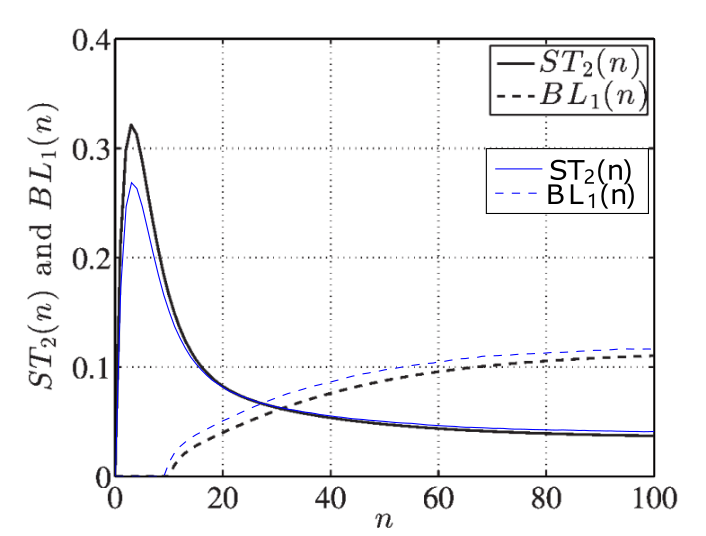
\includegraphics[width=0.5\linewidth]{2_c.png}
	\caption{Performance contrast of a two-machine geometric line $ST_2(n) \ and\ BL_2(n)$}
	\label{2_c}
\end{figure*}

\begin{figure*}[!h]
	\centering
	\subfigure[]{
		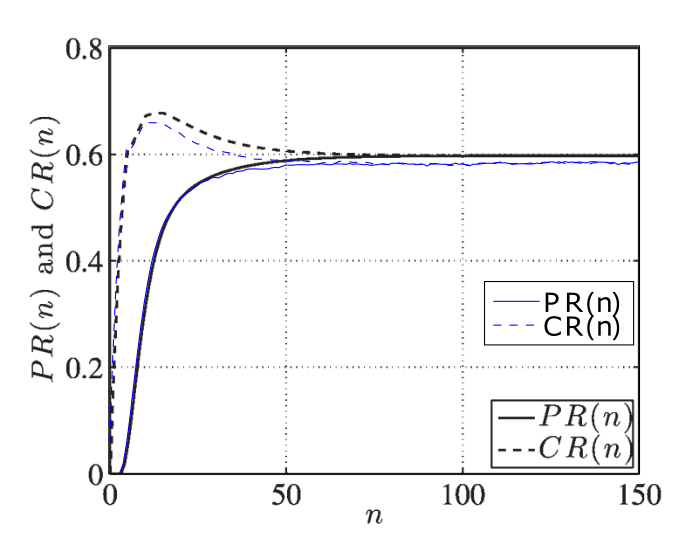
\includegraphics[width=0.45\linewidth,height=0.35\linewidth]{4_a.png}
		\label{d four machine pr and cr}}
	\subfigure[]{
		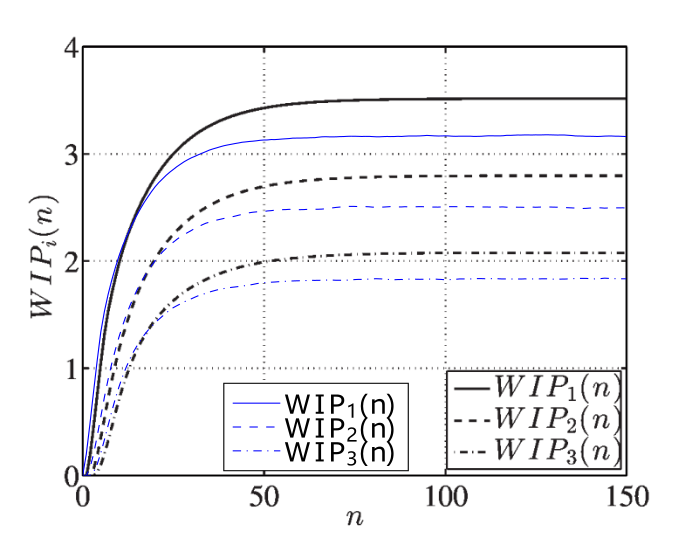
\includegraphics[width=0.45\linewidth,height=0.35\linewidth]{4_b.png}	
		 \label{d four machine wip}}
	\subfigure[]{
		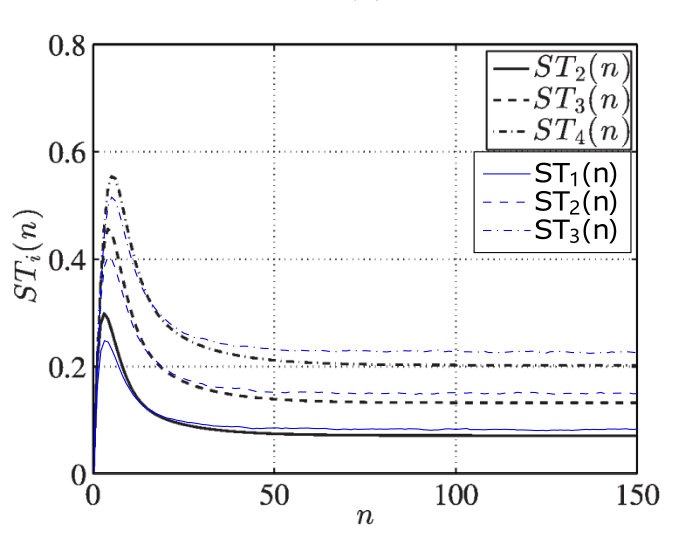
\includegraphics[width=0.45\linewidth,height=0.35\linewidth]{4_c.png}	
		\label{d four machine st}}
	\subfigure[]{
		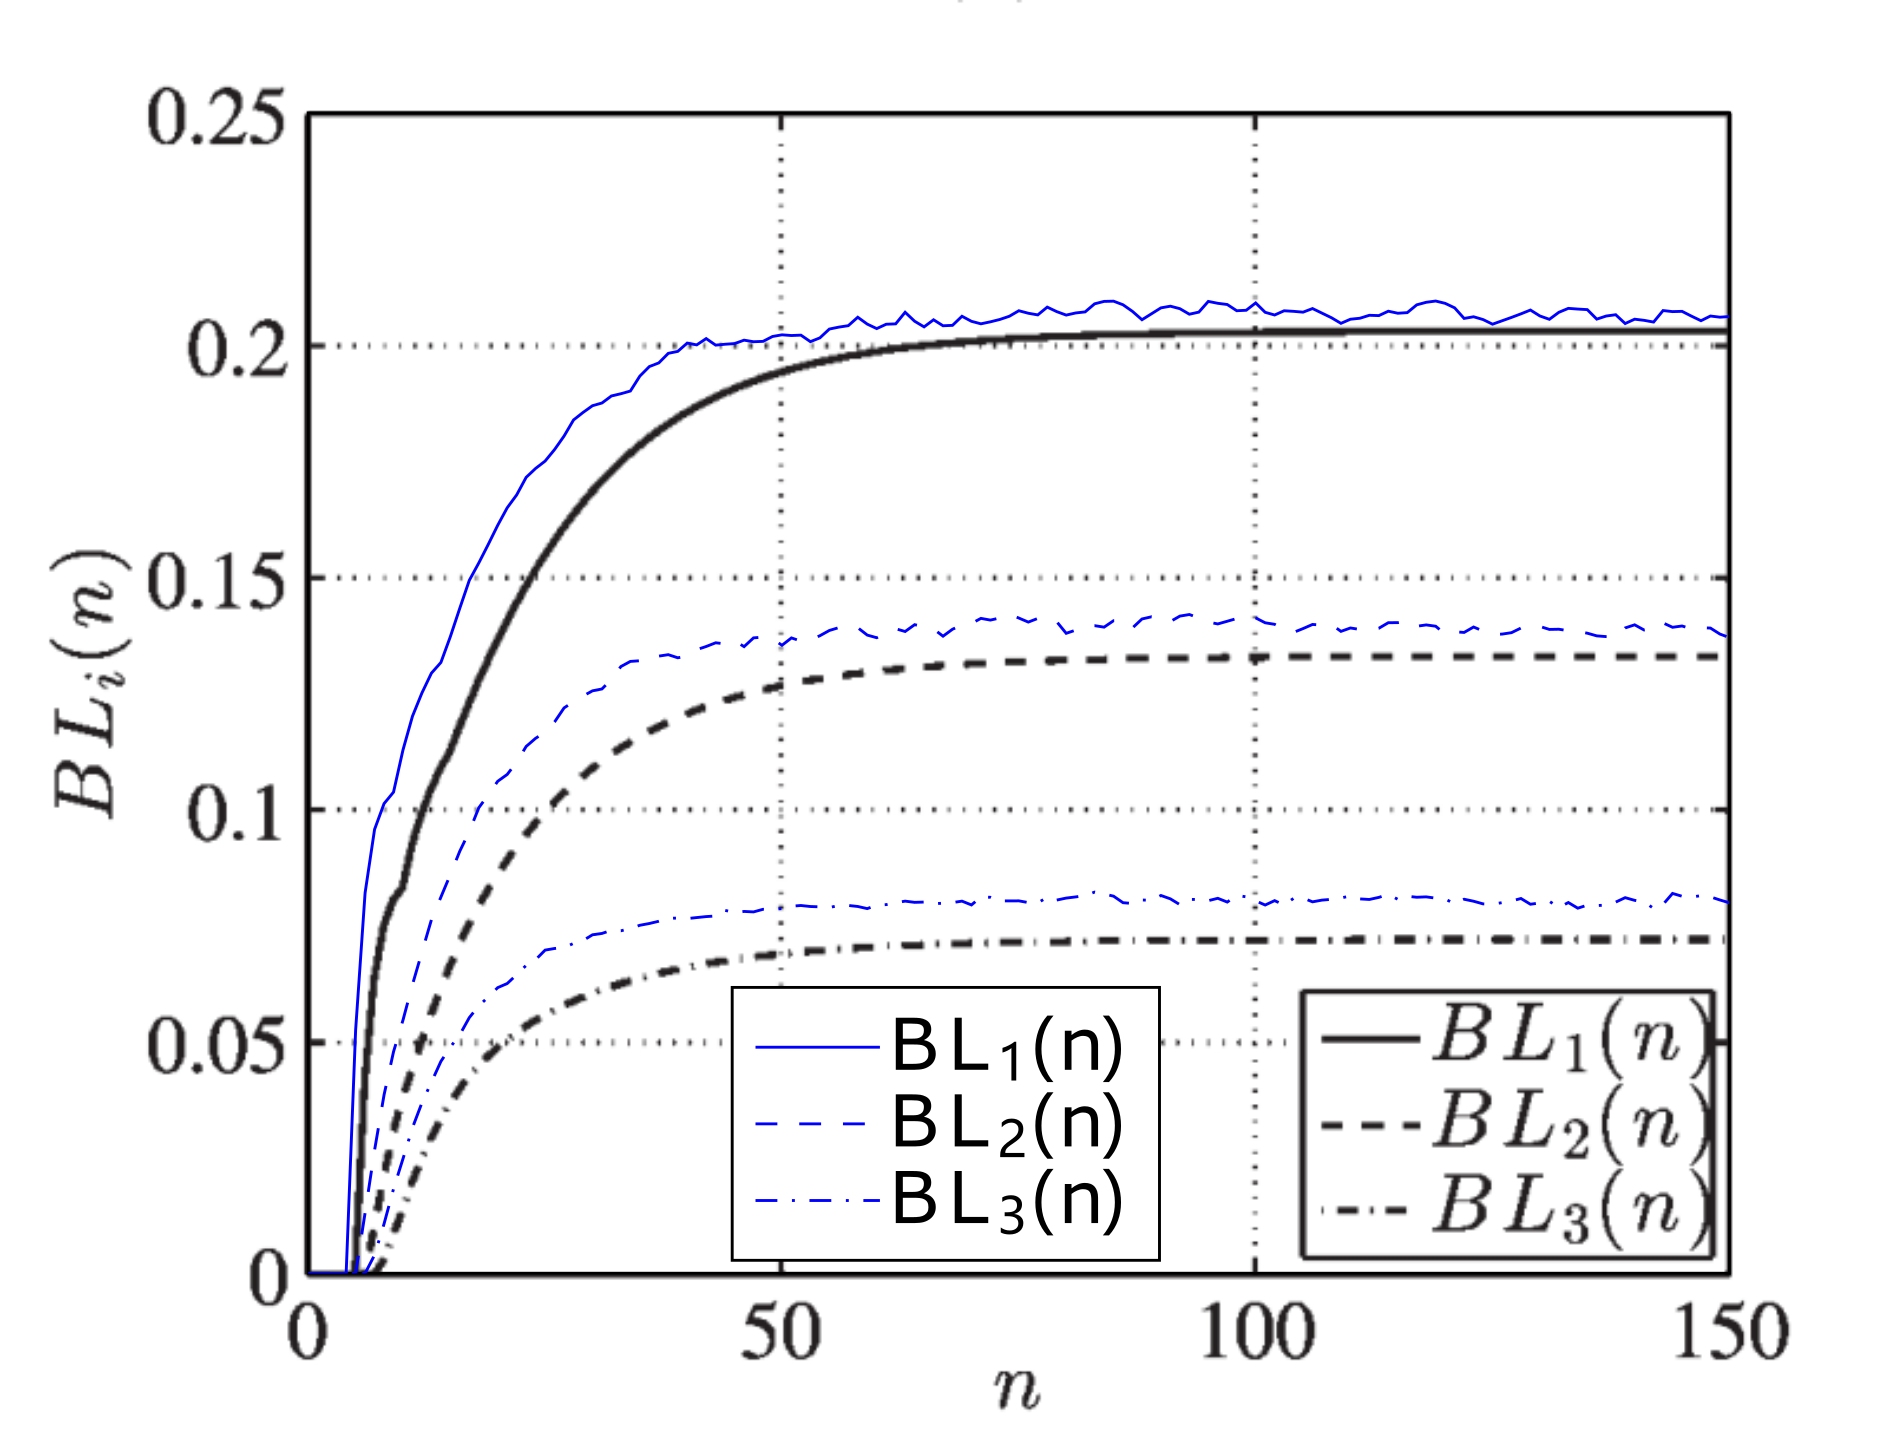
\includegraphics[width=0.45\linewidth,height=0.35\linewidth]{4_d.png}	
		\label{d four machine bl}}
	\caption{Transients of a four-machine geometric line. (a) $PR(n) \ and\ CR(n)$;(b) $WIP(n)$; (c) $ST_i(n)$;(d) $BL_i(n)$.}
	\label{differece four}
\end{figure*}

For the reasons of these difference, we suppose a few points: First, we doubt that whether the lack of enough quantity of samples cause the problem. But when we enlarege the quantity of simulation time from 10000 to 100000, we found no apparent difference from the result. Second, due to that we don't know what kind of programming language the reseachers coding with, a probable cause may be we take a different platform to programm with, and that may cause some accuracy problem. Third, we also doubt that the researchers may do some kind of curve smoothing in oder to present a perfect result.